%%%%%%%%%%%%%%%%%%%%%%%%%%%%%%%%%%%%%%%%%%%%%%%%%%%%%%%%%%%%%%%%%%%%%%
% Lớp 11 | Quan hệ vuông góc trong không gian | Góc giữa đường thẳng và mặt phẳng. Góc nhị diện
% Dạng 1H8?6-6: Khoảng cách giữa 2 đường chéo nhau, biết trước góc (𝑑, (𝑃))
% Số câu: 2  (sinh tự động bởi tach_cau.py; từ nay thầy sửa trực tiếp file này)
%%%%%%%%%%%%%%%%%%%%%%%%%%%%%%%%%%%%%%%%%%%%%%%%%%%%%%%%%%%%%%%%%%%%%%

%%%%%%%%%%%%%%%% ĐÚNG/SAI %%%%%%%%%%%%%%%%

% nguồn: Ok_dungsai_lop11_Lan1
\begin{ex}%[1H8V6-6]%[ma:1dc68ec8]
 Cho lăng trụ đứng $ABC.A' B' C'$ có $AC=a$, $BC=2a$, $\widehat{ACB}=120^{\circ}$. Gọi $M$ là trung điểm của $BB'$. Khi đó, các mệnh đề sau \textbf{ĐÚNG} hay \textbf{SAI}  ?
 \choiceTF 
  {\True $\mathrm{d}\left(CC', \left(ABB' A'  \right)\right)=\dfrac{a\sqrt{21}}{7}$}
   {$\mathrm{d}\left(CC', AM\right)=\dfrac{a\sqrt{21}}{12}$}
  {\True $AA' \perp (ABC)$, $AA' \perp \left(A' B' C'  \right)$}
  {\True Biết khoảng  cách giữa hai mặt đáy lăng trụ bằng $2a$. Khi đó thể tích khối lăng trụ là $a^3\sqrt{3}$}
 \loigiai{ 
  \begin{center}
   \begin{tikzpicture}[scale=1,font=\footnotesize,line join=round,line cap=round,>=stealth]
     \path 
      (0,3) coordinate[label=left: A'] (A') 
      (0,0) coordinate[label=above right:  A] (A)
      (3,0) coordinate[label=right:  C] (C)
      (3,3) coordinate[label=right: C'] (C') 
      (-1,2)  coordinate[label=left: B'] (B')
      (-1,-1)  coordinate[label=left: B] (B)
       ($(B)!.5!(B')$) coordinate[label=left: M] (M);
     \draw  (A')--(B')--(C')--cycle;
     \draw (B)--(B')--(C')--(C)--cycle; 
      \draw[dashed] (A')--(A)--(B)
       (A)--(C);
     \draw[dashed]  (M)--(A);
    \end{tikzpicture}
  \end{center}
  \begin{itemchoice}
   \itemch  Đúng.
   Ta có $CC' \parallel BB' \Rightarrow CC' \parallel \left(ABB'  A' \right)$ nên $d\left(CC', \left(ABB' A' \right)\right)=\mathrm{d}\left(C,\left(ABB' A' \right)\right)$.
   Trong mặt phẳng $(ABC)$, kẻ  $CH\perp AB$ tại $H$. $\quad (1)$
   Vì $ABC.A' B' C'$ là hình lăng trụ đứng nên $AA' \perp (ABC) \Rightarrow  CH\perp AA'$. (2)
   Từ (1) và (2) suy ra $CH\perp \left(ABB' A' \right)\Rightarrow \mathrm{d}\left(C,\left(ABB' A'  \right)\right)=CH$.
   Xét tam giác $ABC$, có $AB^2=CA^2+CB^2-2CA\cdot CB\cdot  \cos 120^{\circ}=7a^2$ $\Rightarrow AB=a\sqrt{7}$.
   Diện tích tam giác $ABC$ là $S_{\triangle ABC}=\dfrac{1}{2} CA\cdot CB\cdot \sin C=\dfrac{1}{2} AB\cdot CH$ 
    $\Rightarrow CH=\dfrac{CA\cdot CB\cdot \sin 120^{\circ}}{AB}=\dfrac{a\cdot 2a\cdot \dfrac{\sqrt{3}}{2}}{a\sqrt{7}}=\dfrac{a\sqrt{21}}{7}$.
   Vậy $\mathrm{d}\left(CC', \left(ABB'  A' \right)\right)=CH=\dfrac{a\sqrt{21}}{7}$.
   \itemch Sai. 
   Ta có $AM$ và $CC'$ là hai đường thẳng chéo nhau mà $\heva{&CC' \parallel \left(ABB' A'  \right) \\ &AM\subset \left(ABB' A' \right)}$
   nên $\mathrm{d}\left(CC', AM\right)=\mathrm{d}\left(CC', \left(ABB' A' \right)\right)=\dfrac{a\sqrt{21}}{7}$. 
    \itemch Đúng.
   Vì $ABC. A' B' C'$ là hình lăng trụ đứng nên $AA' \perp  (ABC)$, $AA' \perp \left(A' B' C' \right)$.
   Do vậy $\mathrm{d}\left((ABC),\left(A' B' C' \right)\right)=AA'=2a$. 
    \itemch Đúng.
   Khối lăng trụ $ABC.A' B' C'$ có chiều cao $h=AA'=2a$, diện  tích đáy là:
   \[S=S_{ABC}=\dfrac{1}{2} CA\cdot CB\cdot \sin  120^{\circ}=\dfrac{1}{2} a\cdot 2a\cdot \dfrac{\sqrt{3}}{2}=\dfrac{a^2\sqrt{3}}{2}.\]
   Thể tích khối lăng trụ là:  $V=Sh=\dfrac{a^2\sqrt{3}}{2} \cdot 2a=a^3\sqrt{3}$.
  \end{itemchoice}
  }
\end{ex}

% nguồn: Ok_dungsai_lop11_Lan1
\begin{ex}%[1H8C6-6]%[ma:8159eddb]
 Cho hình chóp $S.ABCD$ có đáy $ABCD$ là hình chữ nhật với $AB=a\sqrt{2}$,\hfill \, $AC=a\sqrt{3}$. Cạnh bên $SA=2a$ và vuông góc với mặt đáy $(ABCD)$. Khi đó, các mệnh đề sau \textbf{ĐÚNG}  hay \textbf{SAI} ?
 \choiceTF 
   {\True $AD\parallel (SBC)$}
  {Khoảng cách từ $D$ đến mặt phẳng $(SBC)$ bằng $\dfrac{a\sqrt{3}}{3}$} 
  {\True Khoảng cách  giữa hai đường thẳng $SD$, $AB$ bằng $\dfrac{2a\sqrt{5}}{5}$}
  {Thể  tích khối chóp $S.ABCD$ bằng $\dfrac{\sqrt{2} a^3}{3}$}
  \loigiai{
  \begin{center}
   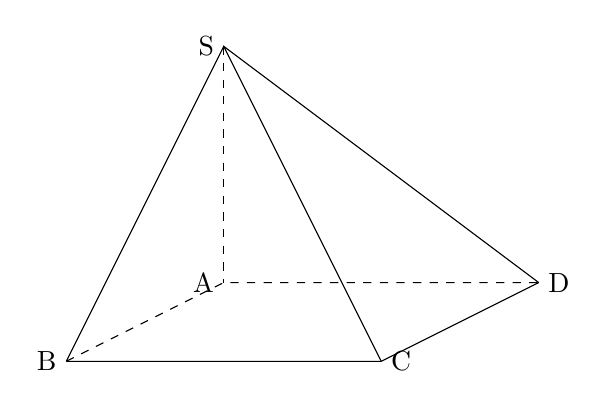
\begin{tikzpicture}
     \path 
      (0,3) coordinate[label=left: S]  (S)
      (0,0) coordinate[label=left:  A] (A)
      (2,-1) coordinate[label=right: C] (C) 
      (4,0) coordinate[label=right:  D] (D)
      (-2,-1)  coordinate[label=left: B] (B);
      \draw (D)--(C)--(B);
     \draw[dashed]  (B)--(A)--(D);
      \draw[dashed] (S)--(A);
     \draw (B)--(S)--(C) 
      (D)--(S); 
    \end{tikzpicture}
  \end{center}
  \begin{itemchoice}
   \itemch  Đúng.
   Ta  có $AD\parallel BC\Rightarrow AD\parallel (SBC)$
   \itemch Sai. 
   Ta có $ \mathrm{d}(D,(SBC))= \mathrm{d}(A,(SBC))$. 
   Trong  mặt phẳng $(SAB)$, kẻ $AH\perp SB$ tại $H$. \hfill{(1)}
   Ta có $\heva{&BC\perp AB \\ &BC\perp  SA} \Rightarrow BC\perp (SAB)\Rightarrow AH\perp BC.$. \hfill{(2)}
   Từ $(1)$ và $(2)$ suy ra $AH\perp (SBC)$ hay  $ \mathrm{d}(A,(SBC))=AH$.
   Tam giác  $SAB$ vuông tại $A$ có đường cao $AH$ nên:
   \[\dfrac{1}{AH^2}=\dfrac{1}{SA^2}+\dfrac{1}{AB^2} \Rightarrow  AH=\dfrac{SA\cdot AB}{\sqrt{SA^2+AB^2}}=\dfrac{2a\cdot a\sqrt{2}}{\sqrt{4a^2+2a^2}}=\dfrac{2a\sqrt{3}}{3}.\]
   Vậy $d(D,(SBC))=d(A,(SBC))=AH=\dfrac{2a\sqrt{3}}{3}$. 
    \itemch Đúng.
   Trong mặt phẳng $(SAD)$, kẻ $AK\perp SD$ tại $K$.  \hfill{(3)}
   Ta có $\heva{&AB\perp SA \\ &AB\perp AD} \Rightarrow AB\perp (SAD)\Rightarrow AB\perp  AK$.\hfill{(4)}
   Từ (3) và (4) suy ra $AK$ là đường vuông góc chung của hai đường thẳng  chéo nhau $AB$, $SD$.
    Tam giác $ACD$ vuông tại $D$ nên $AD=\sqrt{AC^2-CD^2}=\sqrt{3a^2-2a^2}=a$.
   Tam giác $SAD$ vuông tại $A$ có đường cao $AK$  nên
    \[\dfrac{1}{AK^2}=\dfrac{1}{SA^2}+\dfrac{1}{AD^2} \Rightarrow AK=\dfrac{SA\cdot AD}{\sqrt{SA^2+AD^2}}=\dfrac{2a\cdot a}{\sqrt{4a^2+a^2}}=\dfrac{2a\sqrt{5}}{5}.\;\]
   Vậy $d(AB,SD)=AK=\dfrac{2a\sqrt{5}}{5}$. 
    \itemch Sai.
   Diện  tích đáy hình chóp là $S_{ABCD}=a\cdot a\sqrt{2}=a^2\sqrt{2}$.
   Thể tích khối chóp  cần tìm là
   $V_{S.ABCD}=\dfrac{1}{3} SA\cdot S_{ABCD}=\dfrac{1}{3} \cdot 2a\cdot a^2\sqrt{2}=\dfrac{2\sqrt{2} a^3}{3} $  (đơn vị thể tích).
  \end{itemchoice}
 } 
\end{ex}
